% !TEX root =  ../main_manuscript.tex 
\section{Introduction}
\label{sec:introduction}
Chronic non-communicable diseases (e.g., cancer, lung, cardiovascular diseases) cause 60--70\% of human deaths worldwide~\citep{world2014global}. Often patients diagnosed with an early-stage disease undergo surveillance \emph{tests} to detect disease \emph{progression} timely. A progression is a non-terminal event, and usually a trigger for treatment and/or removal from surveillance. Typically the benchmark tests used for confirming progression are \emph{invasive}. Some examples of such tests are, biopsies in prostate cancer surveillance~\citep{bokhorst2015compliance}, endoscopies in Barrett's esophagus~\citep{weusten2017endoscopic}, colonoscopies in colorectal cancer~\citep{krist2007timing}, and bronchoscopies in lung transplant~\citep{mcwilliams2008surveillance} patients.

Invasive tests are repeated until progression is observed, typically as per a one-size-fits-all \emph{fixed schedule}, e.g., biannually,~\citep{mcwilliams2008surveillance,bokhorst2015compliance,krist2007timing}. With recurrent tests, progression is always detected with a time delay (Figure~\ref{fig:delay_explanation}). A shorter delay in detecting progression (\emph{benefit}) can provide a larger window of opportunity for curative treatment. However, with a fixed schedule, this means conducting tests frequently. Frequent tests are \textit{burdensome} as they may cause pain and/or severe medical complications~\citep{loeb2013systematic,krist2007timing}. Consequently, patients may not always comply with frequent tests~\citep{bokhorst2015compliance, LeClercq2015325}. In this regard, since one-size-fits-all fixed schedules do not differentiate between fast and slow/non-progressing patients (large proportion in some diseases), they often have a skewed burden-benefit ratio.

\begin{figure}
\centerline{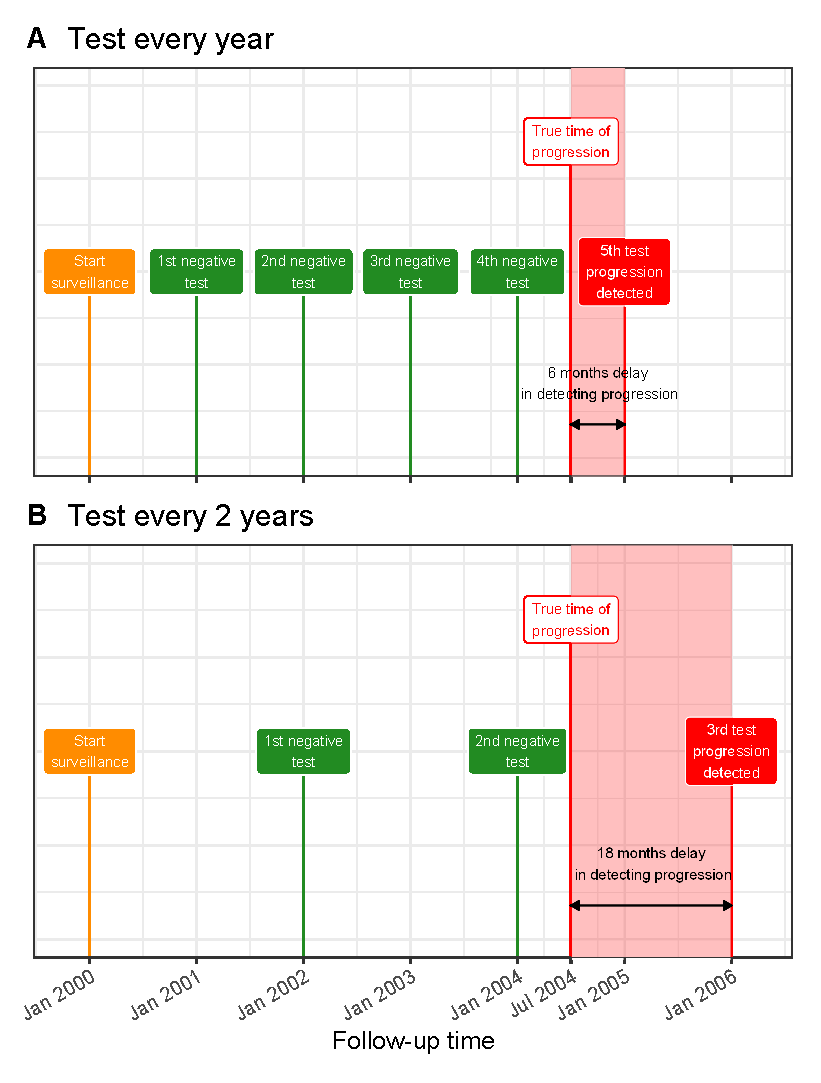
\includegraphics{images/delay_explanation.eps}}
\caption{\textbf{Goal: Finding the optimal tradeoff between the number of invasive tests (burden) and time delay in detecting progression (shorter is beneficial)}. A progression is a non-terminal event in the surveillance of early-stage chronic non-communicable diseases. The true time of progression for the patient illustrated in this figure is July 2004. Since invasive tests are conducted repeatedly, progression is interval-censored and always observed with a delay. Frequent periodical invasive tests in \textbf{Panel~A} lead to a shorter time delay in detecting progression than infrequent periodical invasive tests in \textbf{Panel~B}. The interval-censored time of progression is Jan~2004--Jan~2005 in \textbf{Panel~A} and between Jan~2004--Jan~2006 in \textbf{Panel~B}.} 
\label{fig:delay_explanation}
\end{figure}

The goal of this work (Figure~\ref{fig:delay_explanation}) is to optimize the number of invasive tests and the time delay in detecting progression better than fixed schedules. Specifically, we intend to \emph{personalize} test schedules using patients' clinical data accumulated over surveillance follow-up. This data includes baseline characteristics; previous invasive test results; and longitudinal outcomes such as biomarkers, physical examination, and medical imaging measurements. Previous attempts at personalized scheduling can be divided into three categories. First, heuristic approaches such as decision making flowcharts~\citep{bokhorst2015compliance,weusten2017endoscopic}. However, flowcharts discretize continuous clinical outcomes, often exploit only the last measurement, and ignore the measurement error in observed data. Second, partially observable Markov decision processes~\citep{alagoz2010operations, steimle2017markov} for personalizing test decisions. Although the curse of dimensionality limits their application with continuous longitudinal outcomes. Third, personalized schedules may be obtained by optimizing an explicit utility function of the clinical parameters of interest~\citep{bebu2017optimal,rizopoulos2015personalized}, including our previous work on scheduling biopsies in prostate cancer~\citep{tomer2019personalized,tomer2020webapp}. In this work, we will employ the third approach.

Our solution is as follows. We first develop a full specification of the joint distribution of the patient-specific longitudinal outcomes and the time of progression. To this end, we utilize joint models for time-to-event and longitudinal data~\citep{tsiatis2004joint,rizopoulos2012joint} because they are inherently personalized. Specifically, joint models utilize patient-specific random effects~\citep{mcculloch2005generalized} to model longitudinal outcomes without discretizing them. Subsequently, we input the accumulated clinical data of a new patient into the fitted model to obtain their patient-specific cumulative-risk of progression at their current and future follow-up visits. We then create personalized schedules by planning tests on future visits where the predicted conditional cumulative-risk is above a particular \emph{threshold} (e.g., 5\% risk). We automate the choice of this threshold and the resulting schedule. In particular, we optimize a utility function of the expected number of tests (burden) and time delay in detecting progression (shorter is beneficial) for personalized schedules based on different risk thresholds. We estimate these two quantities for any given schedule in a patient-specific manner using the predicted risk profile of the patient. Hence, patients/doctors can compare the consequences of opting for personalized versus fixed schedules objectively.

%\subsection{Motivational Study}
%\label{subsec:motivational_study}
Our motivation comes from the problem of scheduling biopsies in the world's largest prostate cancer surveillance, called prostate cancer research international active surveillance~\citep{bokhorst2015compliance}, or PRIAS. It has 7813 patients (1134 progressions) with 104904 longitudinal measurements~\citep{tomer2020webapp}. These patients have low/very-low grade cancer, often over-diagnosed due to prostate-specific antigen (PSA) based screening~\citep{loeb2014overdiagnosis}. Surveillance aims to delay serious treatments (e.g., surgery, radiotherapy) until progression is observed. Consequently, patients are monitored routinely via PSA (ng/mL), digital rectal examination or DRE (tumor shape/size), and biopsy Gleason grade group~\citep{epsteinGG2014}. Among these, a biopsy Gleason grade group~$\geq$ 2 is the reference test for confirming progression. Most often, biopsies are scheduled annually~\citep{loeb2014heterogeneity}. However, such a frequent schedule can put an unnecessary burden on patients with slow/non-progressing cancers and cause non-compliance~\citep{bokhorst2015compliance}. Since prostate cancer has the second-highest incidence among all cancers in males~\citep{GlobalCancerStats2012}, individualized biopsy schedules can reduce the burden of biopsies in numerous patients worldwide.

The remaining paper is as follows. Section~\ref{sec:jointmodel} introduces the joint modeling framework. We describe the personalized scheduling methodology in Section~\ref{sec:schedule}, and demonstrate them for prostate cancer surveillance patients in Section~\ref{sec:results}. In Section~\ref{sec:sim_study}, we compare personalized and fixed schedules via a simulation study based on a joint model fitted to the PRIAS dataset.